\section{Auswertung}
\label{sec:Auswertung}

\subsection{Fehlerrechnung}
\label{sec:Fehlerrechnung}
Für die Fehlerrechnung werden folgende Formeln aus der Vorlesung verwendet.
für den Mittelwert gilt
\begin{equation}
    \overline{x}=\frac{1}{N}\sum_{i=1}^N x_i ß\; \;\text{mit der Anzahl N und den Messwerten x} 
    \label{eqn:Mittelwert}
\end{equation}
Der Fehler für den Mittelwert lässt sich gemäß
\begin{equation}
    \increment \overline{x}=\frac{1}{\sqrt{N}}\sqrt{\frac{1}{N-1}\sum_{i=1}^N(x_i-\overline{x})^2}
    \label{eqn:FehlerMittelwert}
\end{equation}
berechnen.
Wenn im weiteren Verlauf der Berechnung mit der fehlerhaften Größe gerechnet wird, kann der Fehler der folgenden Größe
mittels Gaußscher Fehlerfortpflanzung berechnet werden. Die Formel hierfür ist
\begin{equation}
    \increment f= \sqrt{\sum_{i=1}^N\left(\frac{\partial f}{\partial x_i}\right)^2\cdot(\increment x_i)^2}.
    \label{eqn:GaussMittelwert}
\end{equation}
 
\subsection{Invertierender Linearverstärker}
\label{sec:InvertinAmpl}
 
Es wurden drei verschiedene Frequenzverhältnisse $\frac{R_2}{R_1}$ verwendet, zu welchen dann jeweils die Ausgangsamplituden in Abhängigkeit der Frequenz notiert wurden.
Die theoretischen Vergleichswerte für die Leerlaufverstärkung ergeben sich so zum

\begin{align*}
    V_{\text{1,t}} &= \frac{100\,\unit{\kilo\ohm}}{1\,\unit{\kilo\ohm}} =100\\
    V_{\text{2,t}} &= \frac{68\,\unit{\kilo\ohm}}{1\,\unit{\kilo\ohm}} =68\\
    V_{\text{3,t}} &= \frac{150\,\unit{\kilo\ohm}}{1\,\unit{\kilo\ohm}} =150
\end{align*}

Für die Verhältnisse ergeben sich folgende experimentell bestimmte Werte.

\subsubsection{Invertierender Linearverstärker 1}
\label{sec:InvertierenderLinearverstärker1}

\begin{table}
    \centering
    \caption{Messwerte des Invertierenden Linearverstärkers mit $R_1=1\,\unit{\kilo\ohm}$ und $R_2=100\,\unit{\kilo\ohm}$}
    \begin{tabular}{c c c c}
        \toprule
        Frequenz $f\mathbin{/}\unit{\hertz}$ & Ausgangsampl. $U_0\mathbin{/}\unit{\volt}$& Eingangsampl. $U_{\text{i}}\mathbin{/}\unit{\volt}$ & Phasenverschiebung $\mathbin{/}$ rad\\
        \midrule
        5	&19.5	&0.21&	3.14\\
        30&	19.5	&0.21&	3.14\\
        60&	19.5	&0.21&	3.14\\
        120&	19.5&	0.21&	3.14\\
        240&	19.5&	0.21&	3.14\\
        480	&19.5	&0.21&	3.14\\
        960	&19.5	&0.21&	3.05\\
        1920&	19.2&	0.21&	2.97\\
        3840&	18.2&	0.21&	2.74\\
        7680&	14.9&	0.21&	2.34\\
        15280&	8.8&	0.21&	1.83\\
        30480&	5.1	&0.23& 1.71\\
        60000&	2.9	&0.23&	1.61\\
        120000&	1.6	&0.23&	1.43\\
        240000&	1.2	&0.23&	1.22\\
        \bottomrule
    \end{tabular}
    \label{tab:InvAmp1}
\end{table}
Wenn diese Messwerte doppel-logarithmisch aufgetragen werden, folgt der in \autoref{fig:graphInvertAmp1} dargestellte Verlauf des Verhältnisses $U_0/U_{\text{i}}$ in Abhängigkeit der Frequenz $f$.

\begin{figure}
    \centering
    \includegraphics[width=0.8\textwidth]{build/Invertieren1.pdf}
    \caption{Verstärkung $U_A/U_E$ des ersten Invertierenden Linearverstärkers in Abhängigkeit von der Frequenz.}
    \label{fig:inv1plot}
\end{figure}
Deutlich zu sehen ist hier, dass bei kleinen Frequenzen (großer Wert des Logarithmus) nahezu keine Steigung existiert. Wenn  die Verhältnisse $U_0(f)/U_{\text{i}}$ über diese  Werte gemittelt werden, kann die Leerlaufverstärkung ermittelt werden.
Für die Verstärkung folgt so 
\begin{equation*}
    V_1=\frac{U_0}{U_{\text{i}}}= 92.9  \; .
\end{equation*}

Wenn nun ein linearer Fit der Form 
\begin{equation*}
    h'(f)=m\cdot f+b
\end{equation*}
angewendet wird, bzw. in diesem Fall die auf die doppel-logarithmische Skala angepasste Version, 
\begin{equation*}
    h(f)= m \cdot \ln\left({f}\right) + b
\end{equation*}
lassen sich folgende Fit-Parameter bestimmen.
\begin{align*}
    m=&-0.77\pm 0.05 \\
    b=& 11.0\pm 0.5\\
\end{align*}
Die Grenzfrequenz, welche als $f_{1\text{,g}}=\frac{V_1}{\sqrt{2}}$ definiert ist, kann über
\begin{align*}
   ln{\left(\frac{V_1}{\sqrt{2}}\right)}=&m\cdot \ln{\left(f_{1\text{,g}}\right)}+b\\
   \rightarrow f_{1\text{,g}}=&\exp{\left[\ln{\left(\frac{V_1}{\sqrt{2}}\right)-\frac{b}{m}}\right]}\\
\end{align*}
bestimmt werden.
%Für den ersten Invertierenden Linearverstärker ergibt sich so die Grenzfrequenz und daraus die 


\subsubsection{Invertierender Linearverstärker 2}
\label{sec:InvertierenderLinearverstärker2}

\begin{table}
    \centering
    \caption{Messwerte des Invertierenden Linearverstärkers mit $R_1=1\,\unit{\kilo\ohm}$ und $R_2=68\,\unit{\kilo\ohm}$}
    \begin{tabular}{c c c c}
        \toprule
        Frequenz $f\mathbin{/}\unit{\hertz}$ & Ausgangsampl. $U_0\mathbin{/}\unit{\volt}$& Eingangsampl. $U_{\text{i}}\mathbin{/}\unit{\volt}$ & Phasenverschiebung $\mathbin{/}$ rad\\
        \midrule
        15&	27.0&	0.44&	3.14\\		    
        30&	27.0&	0.44&	3.12\\		
        60&	27.0&	0.44&	3.12\\		
        120&	27.0&	0.44&	3.09\\		
        240&	27.0&	0.44&	3.09\\		
        480	&27.0&	0.44&	3.09\\		
        960	&27.0&	0.44&	3.07\\		
        1900&	26.6&	0.44&	3.00\\	
        3800& 26.3&	0.44&	2.83\\	
        7700&	20.5&	0.44&	2.25\\	
        15000&	10.8&	0.44&	1.73\\	
        30000&	5.3&	0.44&	1.41	\\	
        60000&	3.1	&0.44&	1.31	\\	
        120000&	1.7	&0.44&	1.22	\\	
        240000&	1.3	&0.44&	1.13	\\
        \bottomrule
    \end{tabular}
    \label{tab:InvAmp2}
\end{table}
Die Auswertung und Bestimmung der wesentlichen Charakteristika der folgenden Invertierenden Linearverstärker erfolgt in Gänze analog zu jenen in \autoref{sec:InvertierenderLinearverstärker1} durchgeführten Methoden.
Für die Leerlaufverstärkung folgt
\begin{equation*}
    V_2= 61.4\; .
\end{equation*}
\begin{figure}
    \centering
    \includegraphics[width=0.8\textwidth]{build/Invertieren2.pdf}
    \caption{Verstärkung $U_A/U_E$ des zweiten Invertierenden Linearverstärkers in Abhängigkeit von der Frequenz.}
    \label{fig:inv2plot}
\end{figure}
Die Fit-Parameter der blauen Kurve aus \autoref{fig:inv2plot} ergeben sich zu
\begin{align*}
    m=&-0.80\pm 0.01 \\
    b=& 4.18\pm 0.13\; .
\end{align*}
Hieraus folgt für die Grenzfrequenz
\begin{equation*}
    f_{2\text{,g}}=
\end{equation*}
\subsubsection{Invertierender Linearverstärker 3}
\label{sec:InvertierenderLinearverstärker3}

\begin{table}
    \centering
    \caption{Messwerte des Invertierenden Linearverstärkers mit $R_1=1\,\unit{\kilo\ohm}$ und $R_2=150\,\unit{\kilo\ohm}$}
    \begin{tabular}{c c c c}
        \toprule
        Frequenz $f\mathbin{/}\unit{\hertz}$ & Ausgangsampl. $U_0\mathbin{/}\unit{\volt}$& Eingangsampl. $U_{\text{i}}\mathbin{/}\unit{\volt}$ & Phasenverschiebung $\mathbin{/}$ rad\\
        \midrule
        15& 27.0&	0.32&	3.16\\		
        30&	27.0&	0.32&	3.14\\		
        60&	27.0&	0.32&	3.14\\		
        120&	27.0&	0.32&	3.14\\		
        240&	27.0&	0.32&	3.14\\		
        480&	26.8&	0.32&	3.05\\		
        960&	26.5&	0.32&	3.02\\		
        1900&	26.5&	0.32&	2.84\\	
        3800&	24.2&	0.32&	2.58\\	
        7700&	16.0&	0.32&	1.95\\	
        15000&	9.5&	0.32&	1.78\\		
        30000&	5.2&	0.32&	1.68\\		
        60000&	3.0&	0.32&	1.43\\	
        120000&	1.8&	0.32&	1.26\\	
        240000&	1.4&	0.32& 1.08	\\
        \bottomrule
    \end{tabular}
    \label{tab:InvAmp3}
\end{table}
Die Leerlaufverstärkung beträgt
\begin{equation*}
    V_3= 84.4\; .
\end{equation*}

\begin{figure}
    \centering
    \includegraphics[width=0.8\textwidth]{build/Invertieren3.pdf}
    \caption{Verstärkung $U_A/U_E$ des dritten invertierenden Linearverstärkers in Abhängigkeit von der Frequenz.}
    \label{fig:inv3plot}
\end{figure}
Die Fit-Parameter der blauen Kurve aus \autoref{fig:inv2plot} ergeben sich zu
\begin{align*}
    m=&-0.72\pm 0.07 \\
    b=& 9.9\pm 0.7\; .
\end{align*}

\newpage

\subsection{Integrator}
Die Messwerte der Eingangs- und Ausgangsspannung in Abhängigkeit der Frequenz befinden sich in \autoref{tab:Integrator}. 
\begin{table}
    \centering
    \caption{Messwerte des Integrators mit $R=10\,\unit{\kilo\ohm}$ und $C=100\,\unit{\nano\farad}$}
    \begin{tabular}{c c c}
        \toprule
        Frequenz $f\mathbin{/}\unit{\hertz}$ & Eingangsspannung $U_{\text{E}}\mathbin{/}\unit{\volt}$& Ausgangsspannung $U_{\text{A}}\mathbin{/}\unit{\volt}$ \\
        \midrule
        7& 3.02 & 28.6 \\
        15 & 3.02 & 26.1 \\
        20 & 3.02 & 20.6 \\
        30 & 3.02 & 15.0 \\
        45 & 3.02 & 10.8 \\
        60 & 3.02 & 8.5 \\
        90 & 3.02 & 6.2 \\
        120 & 3.02 & 4.7 \\
        180 & 3.02 & 3.5 \\
        240 & 3.02 & 2.8 \\
        350 & 3.02 & 2.3 \\
        480 & 3.02 & 1.7 \\
        700 & 3.02 & 1.5 \\
        960 & 3.02 & 1.4 \\
        \bottomrule
    \end{tabular}
    \label{tab:Integrator}
\end{table}
Aus diesen lässt sich mittels \autoref{eqn:verstaerkung} die Verstärkung des Signals berechnen. Diese wird in \autoref{fig:intplot} erneut
in Abhängigkeit der Frequenz dargestellt. Dabei sind beide Achsen logarithmisch. In diesem Fall lässt sich eine Ausgleichsgerade:
\begin{equation}
    ln(v) = m \cdot ln(f) + n
    \label{eqn:ausgleichger}
\end{equation} 
bestimmen, wobei der erste Wert nicht ganz auf der Geraden liegt und deshalb ausgenommen wird. 
\begin{figure}
    \centering
    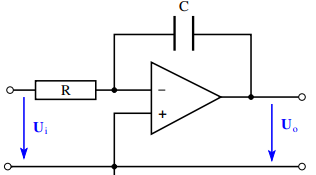
\includegraphics[width=0.8\textwidth]{build/integrator.pdf}
    \caption{Verstärkung $U_A/U_E$ eines Integrators in Abhängigkeit von der Frequenz.}
    \label{fig:intplot}
\end{figure}
Experimentell ergeben sich für die Parameter: 
\begin{align*}
    m &= -0.738 \pm 0.021 \\
    n &= 4.07 \pm 0.10 \\
\end{align*}
Wenn \autoref{eqn:ausgleichger} nun zu 
\begin{equation*}
    V = f^m exp(n)
\end{equation*}
umgestellt und mit \autoref{eqn:int} verglichen wird, ergeben sich folgende Theoriewerte:
\begin{align*}
    m &= -1 \\
    n &= ln(\frac{1}{RC}) = 6.91
\end{align*}


\subsection{Differentiator}
Die Messwerte der Eingangs- und Ausgangsspannung in Abhängigkeit der Frequenz für den Differentiator befinden sich in \autoref{tab:Differentiator}.
\begin{table}
    \centering
    \caption{Messwerte des Differentiators mit $R=100\,\unit{\kilo\ohm}$ und $C=22\,\unit{\nano\farad}$}
    \begin{tabular}{c c c}
        \toprule
        Frequenz $f\mathbin{/}\unit{\hertz}$ & Eingangsspannung $U_{\text{E}}\mathbin{/}\unit{\volt}$& Ausgangsspannung $U_{\text{A}}\mathbin{/}\unit{\volt}$ \\
        \midrule
        7& 6.15 & 1.1 \\
        15 & 5.99 & 1.6 \\
        20 & 5.99 & 2.1 \\
        30 & 5.99 & 2.9 \\
        45 & 6.15 & 3.9 \\
        60 & 5.99 & 5.3 \\
        90 & 5.99 & 7.8 \\
        120 & 5.99 & 11.5 \\
        180 & 5.99 & 14.3 \\
        240 & 5.99 & 19.1 \\
        350 & 5.99 & 27.1 \\
        \bottomrule
    \end{tabular}
    \label{tab:Differentiator}
\end{table}
Auch diesmal wird die Verstärkung $V=U_A/U_B$ in Abhängigkeit von der Frequenz doppellogarithmisch geplottet. Die Ausgleichsgerade 
ergibt sich erneut über \autoref{eqn:ausgleichger}. Für diese berechnen sich die Parameter:
\begin{align*}
    m&= 0.869 \pm 0.023\\
    n &=-3.63 \pm 0.10 \\
\end{align*}

\begin{figure}
    \centering
    \includegraphics[width=0.8\textwidth]{build/differentiator.pdf}
    \caption{Verstärkung $U_A/U_E$ eines Differentiators in Abhängigkeit von der Frequenz.}
    \label{fig:diffplot}
\end{figure}
Erneut wird \autoref{eqn:ausgleichger} mit \autoref{eqn:dif} verglichen. Dabei ergeben sich die folgenden Theoriewerte:
\begin{align*}
    m &= 1 \\
    n &= ln(RC) = -6.12
\end{align*}

\subsection{Schmitt-Trigger}
Über die erste Methode wurde ein Schwellenwert von $U_+=3.213 \,\unit{\volt}$ gemessen. Beim Anlegen einer Dreieckspannung wurde als Schwellenwert 
$U_+=2.994\,\unit{\volt}$ gemessen. Wenn aus diesen Werten der Mittelwert gebildet wird, ergibt sich $U_+=3.104\,\unit{\volt}$. Der Theoriewert 
ergibt sich über \autoref{eqn:schwell}. Dabei ist $U_S$ die Ausgangsspannung am Schwellwert, d.h. die Ausgangsspannung springt abrupt auf 
$U_S$

\subsection{Signalgenerator}
In \autoref{fig:genDrei} ist in gelb das sinusförmige Eingangssignal und in grün das dreieckförmige Ausgangssignal dargestellt. 
Desweiteren lassen sich folgende Werte für die Amplituden und die Frequenz ablesen:
\begin{align*}
    Amp_1 &= 3.14 \,\unit{\volt} \\
    Amp_2 &= 18.7 \,\unit{\volt} \\
    f_2 &= 100.4 \,\unit{\hertz} \, .\\
\end{align*}

\begin{figure}
    \centering
    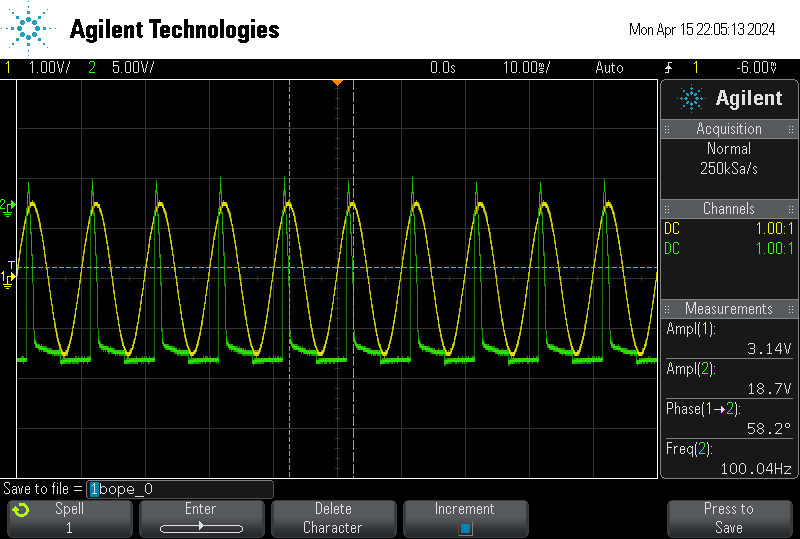
\includegraphics[width=0.8\textwidth]{genDrei.png}
    \caption{Ausgangs- und Eingangssignal eines Signalgenerators.}
    \label{fig:genDrei}
\end{figure}
Mittels \autoref{eqn:fdrei} lässt sich die Frequenz theoretisch berechnen. Es ergibt sich
\begin{equation*}
    f = 2500 \,\unit{\hertz} \, .
\end{equation*}
Auch die Amplitude des Ausgangssignals lässt sich theoretisch berechnen. Es ergibt sich mit \autoref{eqn:amp2}
\begin{equation*}
    Amp_2 = 31.4 \,\unit{\volt}
\end{equation*}

\subsection{Generator mit variierender Amplitude}
Beim Anlegen einer Rechteckspannung, entsteht eine gedämpfte Oszillation. Dies konnte im Versuch mit dem Oszilloskop aufgezeichnet werden und 
wird  in \autoref{fig:genvarosz} abgebildet. Dabei beschreibt die gelbe Linie die Rechteckspannung als Eingangssignal und die grüne Linie 
die gedämpfte Oszillation als Ausgangssignal.
\begin{figure}
    \centering
    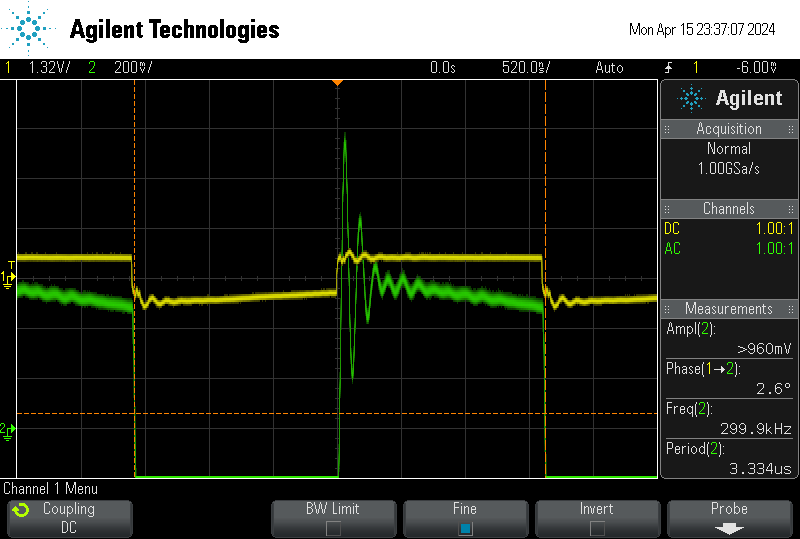
\includegraphics[width=0.7\textwidth]{genvarplot.png}
    \caption{Verlauf der gedämpften Oszillation.}
    \label{fig:genvarosz}
\end{figure}
Nun konnten mithilfe des Oszilloskops die Messdaten extrahiert werden. Bei genauerer Analayse konnten so die Maxima der Ausgangsspannung 
ausfindig gemacht werden. Diese sind in Abhängigkeit von der Zeit in \autoref{fig:genvarAmp} dargestellt.
\begin{figure}
    \centering
    \includegraphics[width=0.8\textwidth]{build/genvar.pdf}
    \caption{Verlauf der Amplituden der gedämpften Oszillation}
    \label{fig:genvarAmp}
\end{figure}